\chapter{Realisierung}
\Blindtext
\newpage
\section{Beispielcode}
%%%% minipage um zu verhinden, dass das Listing durch Figures oder andere floats zerschnitten wird
\begin{minipage}{\linewidth}
\lstinputlisting[language=Java,
	backgroundcolor=\color{lightgray},
	captionpos=b,
	basicstyle=\small,
	numbers=left,
	numberstyle=\tiny,
	frame=TRbl,
	caption=Beispiellisting von JAVA-Code,
	label={lst:example01}]{sections/examples/helloWorld.java}
% Pfade gelten immer von der Hauptdatei aus (Werwolf-Spielleiter-Doku.tex)	
\end{minipage}
%%%% Figures sind floats, LaTeX platziert sie automatisch. Das kann über extra Optionen der figure verhindert werden ( Option [H] aus package float),
%%%% aber da man Figures usw. eh im Text referenzieren muss, reicht es meistens zu prüfen, dass nichts anderes zerschnitten wurde (siehe Codelisting)
\section{Beispielbild}
\begin{figure}[H]
	\centering
	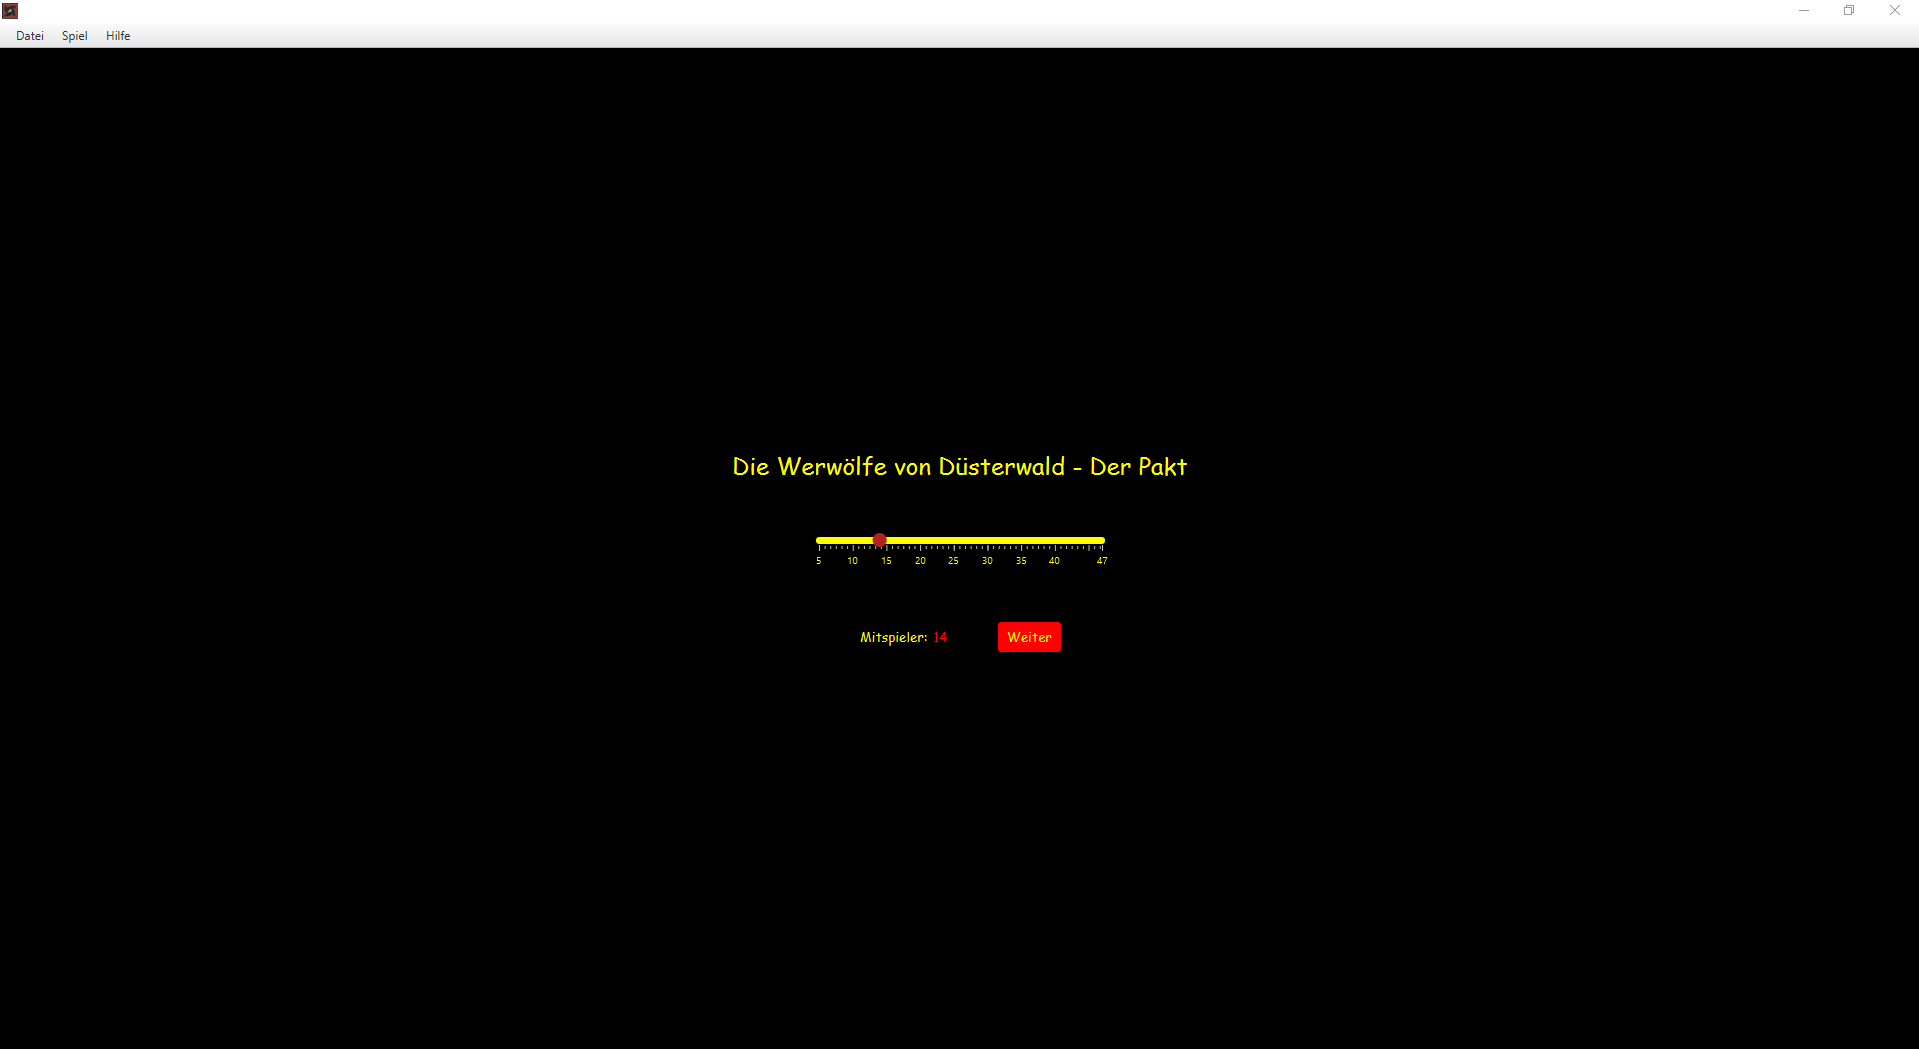
\includegraphics[width=\textwidth]{sections/examples/appStartScreen.png}
	\caption{Startbildschirm des Programms}
	\label{figure:appStartScreen}
\end{figure}
% Beispielreferenzierung auf Element mit label 'figure:appStartScreen'
Wie in Abbildung \ref{figure:appStartScreen} zu sehen...